%   Filename    : chapter_3.tex

\chapter{Research Methodology}

This chapter describes the methodology used in developing and evaluating MitoChime. It covers data collection, read simulation, preprocessing and alignment, feature extraction, classical and deep learning model development, feature importance analysis, ablation testing, threshold-based filtering, downstream assembly validation, and documentation.

\section{Research Activities}

Figure~\ref{fig:process_diagram} summarizes the overall workflow of the study. The process began with the collection of a mitochondrial reference genome of \textit{Sardinella lemuru} from NCBI. This reference was used to simulate both clean and chimeric paired-end Illumina reads. The simulated reads were then aligned to the reference genome, and read-level features associated with chimeric structure were extracted.

These features were used to train and evaluate classical machine learning models for chimera detection. The best-performing classical model, Gradient Boosting (GB), was further examined through feature importance and ablation analyses. Subsequently, sequence-based deep learning models were also developed to assess whether chimeric reads could be identified directly from nucleotide sequences without relying on alignment-derived features. Finally, model predictions were used to filter suspected chimeric reads, and the effect of filtering was assessed through downstream mitochondrial assembly.

\begin{figure}[H]
\centering

\includegraphics[width=0.45\linewidth]{figures/methodology.png}
\caption{Overall workflow of the study.}
\label{fig:process_diagram}
\end{figure}

\section{Data Collection}

The mitochondrial reference genome of \textit{Sardinella lemuru} was obtained from the NCBI database in FASTA format (accession number \texttt{NC\_039553.1}). This sequence served as the reference for simulation and alignment throughout the study.

Because experimentally validated chimeric mitochondrial read datasets were unavailable, simulated data were generated to produce labelled examples of both clean and chimeric reads for supervised learning.

\section{Data Simulation and Preprocessing}

\subsection{Simulation of Clean Reads}

Clean paired-end reads were simulated from the reference genome using \texttt{wgsim}. Reads of length 150 bp were generated to approximate Illumina short-read sequencing data. A total of 10{,}000 paired-end fragments were simulated using the following command format:

\begin{verbatim}
wgsim -1 150 -2 150 -r 0 -R 0 -X 0 -e 0.05 -N 10000 \
       original_reference.fasta clean_R1.fastq clean_R2.fastq
\end{verbatim}

\subsection{Simulation of Chimeric Reads}

Chimeric templates were generated using a custom Python script. Two non-adjacent segments from the mitochondrial reference were selected and concatenated to mimic PCR-induced template switching. Short overlapping regions were optionally retained to represent microhomology near the junction.

The resulting chimeric templates were written to a FASTA file and used as input to \texttt{wgsim} under the same sequencing parameters applied to clean reads, producing 10{,}000 paired-end chimeric fragments.

\subsection{Reference Indexing and Alignment}

Both clean and chimeric reads were aligned to the original mitochondrial reference using \texttt{minimap2}. The reference was first indexed:

\begin{verbatim}
minimap2 -d ref.mmi original_reference.fasta
\end{verbatim}

The simulated reads were then mapped using the short-read preset:

\begin{verbatim}
minimap2 -ax sr -t 8 ref.mmi clean_R1.fastq clean_R2.fastq > clean.sam
minimap2 -ax sr -t 8 ref.mmi chimera_R1.fastq chimera_R2.fastq > chimera.sam
\end{verbatim}

The SAM files were converted to BAM format, sorted, and indexed using \texttt{samtools}:

\begin{verbatim}
samtools view -bS clean.sam -o clean.bam
samtools view -bS chimera.sam -o chimera.bam

samtools sort clean.bam -o clean.sorted.bam
samtools index clean.sorted.bam

samtools sort chimera.bam -o chimera.sorted.bam
samtools index chimera.sorted.bam
\end{verbatim}

Only mapped primary reads were retained for alignment-based feature extraction.

\subsection{Construction of Labelled Datasets}

After preprocessing, reads were assigned class labels and organized into datasets for modelling. Clean reads were labelled as class 0, whereas chimeric reads were labelled as class 1. Separate datasets were prepared for feature-based machine learning and sequence-based deep learning experiments. An illustrative example of one read from the dataset is shown in Figure~\ref{fig:dataset_example}.

\begin{figure}[H]
\centering
\fbox{
\parbox{0.92\textwidth}{
\small
\textbf{Example data point from the dataset}\\[4pt]
\texttt{read\_id: NC\_039553.1\_10001\_10492\_5:0:0\_8:0:0\_b77/1}\\
\texttt{label: 0}\\
\texttt{seq: GTAAGGCATAGTAAGGCAATGGTGAGGCTGTGTGTGATTGCAGCAGTTCAAATTCACT...}
}
}
\caption{Illustrative example of one record from the simulated dataset. The sequence is truncated for readability.}
\label{fig:dataset_example}
\end{figure}


\section{Feature Extraction Pipeline}

A custom feature extraction pipeline was implemented in Python to compute read-level descriptors associated with PCR-induced chimerism from the BAM files. Each row of the resulting TSV matrix represented one read, and each column represented one numeric feature.

The pipeline focused on five feature groups: (1) supplementary alignment and alignment-structure features, (2) soft-clipping and inferred breakpoint features, (3) k-mer composition discontinuity features, (4) microhomology features, and (5) alignment quality features.

\subsection{Supplementary Alignment and Alignment-Structure Features}

For each primary read, the pipeline checked for the presence of the \texttt{SA} tag. If present, the tag was parsed to recover supplementary alignment information, including mapped position, strand, mapping quality, and mismatch count. From this, features such as \texttt{has\_sa}, \texttt{sa\_count}, number of alignment segments, strand consistency, and summary statistics of segment distances and mapping qualities were computed.

\subsection{Soft-Clipping and Breakpoint Features}

Soft-clipped bases were extracted from the Concise Idiosyncratic Gapped Alignment Report (CIGAR) string. Left and right soft-clipped lengths, as well as total clipped bases, were recorded. A candidate breakpoint position was inferred using clipping boundaries where available, or alignment/read midpoints otherwise.
\subsection{Feature Representation}

For the classical machine learning pipeline, a tabular feature matrix was constructed in which each primary-mapped read was represented by a fixed-length numeric feature vector computed using \texttt{pysam} and NumPy. The extracted predictors were organized into several feature families. First, supplementary-alignment and alignment-structure summaries were derived from SA tags, including the presence and count of supplementary alignments, distances between aligned segments, strand consistency, and aggregate alignment statistics such as supplementary-alignment MAPQ and NM values. Second, CIGAR-derived clipping statistics were computed, including left and right soft clipping, total clipped bases, and an inferred breakpoint position. Third, k-mer composition discontinuity between read segments was quantified using \(k=6\), through cosine difference and Jensen--Shannon divergence between the left and right normalized k-mer profiles. Fourth, microhomology descriptors around the inferred breakpoint were extracted, including the longest exact suffix--prefix overlap within a \(\pm 40\) bp window and the GC fraction of the detected overlap. These were complemented by basic alignment-quality indicators such as mapping quality. In total, the resulting classical feature matrix contained 23 numeric predictor variables per read.

In parallel, for the deep learning experiments, the raw nucleotide sequence was retained as a separate input representation. Each read had fixed length \(L=150\), consistent with the simulated read length used throughout the study. For the convolutional neural network, sequences were one-hot encoded during both training and inference using four base channels corresponding to A, C, G, and T. Ambiguous bases were represented as all-zero vectors.

\subsection{K-mer Composition Discontinuity}

To capture compositional shifts consistent with chimeric junctions, each read was divided into left and right segments at the inferred breakpoint, and k-mer composition was compared between the two sides. In this study, \(k=6\) was used. For each segment, normalized 6-mer frequency profiles were computed after excluding ambiguous bases. Two complementary measures were then derived: cosine difference, which summarizes directional dissimilarity between the segment-wise k-mer vectors, and Jensen--Shannon divergence, which quantifies the divergence between the corresponding k-mer distributions. These were recorded as \texttt{kmer\_cosine\_diff} and \texttt{kmer\_js\_divergence}, respectively.

\subsection{Microhomology Features}

A local breakpoint-centered window was examined to characterize short exact overlaps between the left and right sides of a read, which may arise during chimera formation. In the present work, a microhomology search window of \(\pm 40\) bp was used. Within this window, the longest exact suffix--prefix overlap between the left and right segments was identified and recorded as \texttt{microhomology\_length}. The GC content of the detected overlap, when present, was computed and stored as \texttt{microhomology\_gc}. These features were included to assess whether local sequence overlap contributed useful discriminatory signal for chimera detection.

\subsection{Alignment Quality Features}

General alignment quality measures were also incorporated as predictors. These included mapping quality (\texttt{mapq}), which is intended to capture whether chimeric reads exhibit different alignment irregularities relative to clean reads.

\section{Classical Machine Learning Model Development}

The extracted clean and chimeric feature matrices were merged into a single labelled dataset containing 23 numeric features. The dataset was partitioned into training (80\%) and test (20\%) subsets using stratified sampling.

A benchmarking stage was conducted using multiple classification algorithms, including Logistic Regression, linear SVM, \(k\)-Nearest Neighbours, Gaussian Na\"ive Bayes, Random Forest, ExtraTrees, Bagging, Gradient Boosting, XGBoost, LightGBM, CatBoost, Multilayer Perceptron, and a dummy baseline. Model development was performed in Python using \texttt{scikit-learn} and related libraries.

Five-fold stratified cross-validation was used on the training set. Performance was assessed using accuracy, precision, recall, F1-score for the chimeric class, and the area under the receiver operating characteristic curve (ROC--AUC).


\section{Hyperparameter Optimization and Model Evaluation}

Top-performing model families from the initial benchmark were selected for further optimization using randomized search with five-fold stratified cross-validation. Hyperparameters were tuned according to model type, including the number of estimators, depth, learning rate, regularization, and hidden-layer configuration where applicable.

Among the tuned feature-based models, the best validation performance was obtained by a \texttt{GradientBoostingClassifier} from \texttt{sklearn.ensemble}. The selected final configuration used \texttt{n\_estimators = 400}, \texttt{learning\_rate = 0.2}, \texttt{max\_depth = 3}, \texttt{min\_samples\_leaf = 4}, and \texttt{subsample = 1.0}. This model was then refit on the full training split and evaluated once on the held-out test split. Final evaluation on the held-out test set included accuracy, precision, recall, F1-score, ROC--AUC, and confusion matrix analysis. 

\section{Feature Importance and Ablation}

Feature importance analysis was performed using the tuned Gradient Boosting model. Two complementary approaches were applied. First, the model’s built-in feature importance scores were examined to identify predictors that contributed most strongly to the learned decision rules. Second, permutation importance was computed on the held-out test set to assess the effect of disrupting each feature on predictive performance. For interpretability, the predictors were also grouped into conceptual feature families corresponding to alignment structure, soft clipping, k-mer discontinuity, microhomology, and alignment quality.

An ablation analysis was also conducted to examine the contribution of microhomology-related predictors. In this experiment, the features \texttt{microhomology\_length} and \texttt{microhomology\_gc} were removed, and the Gradient Boosting model was retrained under the same modelling procedure. Performance of the ablated model was then compared against that of the full model to determine the extent to which breakpoint-local overlap information contributed to chimera classification.

\section{Deep Learning Model Development}

In addition to feature-based classical machine learning models, sequence-based deep learning models were developed to classify reads directly from nucleotide sequence. Two architectures were implemented in PyTorch: 1D CNN and a BiGRU model.

\subsection{Input Preparation}

For the CNN, each sequence was converted into a one-hot encoded representation with four base channels corresponding to A, C, G, and T. Ambiguous bases were encoded as all-zero vectors. For the BiGRU, sequences were transformed into overlapping k-mer tokens and encoded as integer sequences for embedding-based modelling. In the BiGRU configuration used in this work, \(k=4\) was applied. Since each read had length 150 bp, this produced \(150 - 4 + 1 = 147\) overlapping 4-mer tokens per read.

\subsection{Convolutional Neural Network}

The CNN architecture consisted of three convolutional blocks with 64, 128, and 256 filters, using kernel sizes of 7, 5, and 3, respectively. Rectified linear unit (ReLU) activations were applied after each convolution, and max-pooling was performed after the first two convolutional blocks. The convolutional feature maps were then reduced using adaptive max pooling and passed to a two-layer multilayer perceptron classification head with dimensions \(256 \rightarrow 128 \rightarrow 2\), with dropout set to 0.2.

For the final experiments, the CNN was trained using mini-batches of 128 for up to 30 epochs, with learning rate \(1\times10^{-3}\) and weight decay \(1\times10^{-4}\). Model checkpoint selection was based on the best validation F1-score for the chimeric class. Training and evaluation were performed through the project deep learning pipeline using the sequence TSV files prepared from the labelled dataset.

\subsection{Bidirectional GRU Model}

The BiGRU model was likewise implemented in PyTorch for sequence-based classification using tokenized k-mer input. Each integer-encoded 4-mer sequence was first passed through an embedding layer with embedding dimension 64. The embedded sequence was then processed by a BiGRU encoder with hidden size 256 and one recurrent layer. Bidirectional processing allowed the model to capture contextual dependencies in both forward and reverse sequence directions. The final sequence representation was obtained through last-state pooling and passed to a classification head for binary prediction.

The BiGRU was trained for 30 epochs using a batch size of 128, learning rate \(1\times10^{-3}\), weight decay \(1\times10^{-4}\), and random seed 42. Model selection was based on the validation F1-score of the chimeric class. These same optimization settings were used both during five-fold cross-validation and during final held-out training and evaluation.

\subsection{Training and Evaluation}

Both deep learning models were trained on the same training split used for the classical machine learning experiments and were evaluated on the same held-out test split to ensure comparability across modelling approaches. Model training was performed using mini-batch optimization for multiple epochs, and the final reported checkpoint for each model was the one achieving the best validation F1-score for the chimeric class.

For the CNN, the final reported model was trained using \texttt{PAIR\_train\_seq\_L150.tsv} and evaluated on \texttt{PAIR\_test\_seq\_L150.tsv} with 30 epochs and batch size 128. For the BiGRU, five-fold cross-validation was first conducted on fold-specific training and validation TSV files, after which the final held-out model was trained on the full training split and evaluated on the held-out test split using the same architectural and optimization settings.

\section{Threshold-Based Read Filtering}

The final trained classifiers were also evaluated as practical filtering tools for read cleanup. Each read was assigned a probability of belonging to the chimeric class, and a user-specified threshold \(\tau \in [0,1]\) was used to determine whether the read should be removed. A read pair was retained if its assigned chimeric probability satisfied \(p < \tau\), and removed otherwise.

To preserve mate consistency, filtering was performed at the pair level using a normalized base read identifier, with mate suffixes such as \texttt{/1} and \texttt{/2} removed before matching. This ensured that both mates of a read pair were either retained together or removed together in the output FASTQ files. 

\section{Downstream Assembly Validation}

To evaluate the practical value of filtering, downstream mitochondrial assemblies were generated from both unfiltered and filtered read sets. Assembly results were compared using metrics such as number of contigs, maximum contig length, and graph complexity.

Assemblies were produced using \texttt{SPAdes}. Improvement in assembly quality after filtering was interpreted as evidence that the removed reads were disruptive to mitochondrial reconstruction.

\section{Validation and Comparative Testing}

Validation was conducted using both internal and external evaluation. Internal validation was achieved through five-fold stratified cross-validation on the training data, while external evaluation was performed on the held-out test set.

Comparative testing was performed across classical machine learning and deep learning models to determine which approach provided the best balance of predictive accuracy, interpretability, and downstream utility.

\section{Documentation and Reproducibility}

All scripts, datasets, model outputs, and evaluation results were organized and version-controlled in a GitHub repository. Separate directories were maintained for references, simulated reads, alignments, extracted features, trained models, reports, and filtered outputs.

The computational environment was standardized using Conda, with dependencies recorded in an \texttt{environment.yml} file. Analytical procedures, software versions, and command-line parameters were documented in the project \texttt{README}. Manuscript preparation was carried out using \LaTeX. Figure~\ref{fig:pipeline_cli} shows the command-line execution interface of the MitoChime pipeline used in the study.

\begin{figure}[H]
\centering
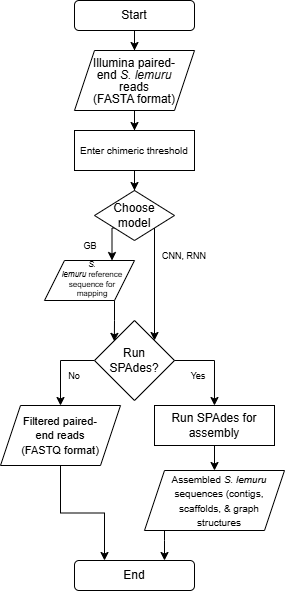
\includegraphics[width=0.4\linewidth]{figures/pipeline.png}
\caption{Command-line execution interface of the MitoChime pipeline.}
\label{fig:pipeline_cli}
\end{figure}

\section{Calendar of Activities}

Table~\ref{tab:project_timeline} presents the overall timetable of activities for the study.

\begin{table}[H]
\centering
\caption{Timetable of activities.}
\label{tab:project_timeline}
\resizebox{\textwidth}{!}{%
\begin{tabular}{|c|c|c|c|c|c|c|c|}
\hline
\textbf{Activities (2025--2026)} & \textbf{Nov} & \textbf{Dec} & \textbf{Jan} & \textbf{Feb} & \textbf{Mar} & \textbf{Apr} & \textbf{May} \\
\hline
Data Collection and Simulation & $\bullet\bullet\bullet\bullet$ & & & & & & \\
\hline
Alignment and Feature Extraction & $\bullet$ & $\bullet\bullet\bullet$ & & & & & \\
\hline
Classical ML Development and Benchmarking & & $\bullet$ & $\bullet\bullet\bullet$ & $\bullet\bullet\bullet$ & & & \\
\hline
Hyperparameter Tuning, Feature Importance, and Ablation & & & & $\bullet$ & $\bullet\bullet\bullet$ & $\bullet$ & \\
\hline
Deep Learning Development & & & $\bullet$ & $\bullet\bullet\bullet$ & $\bullet\bullet$ & & \\
\hline
Filtering and Assembly Validation & & & & & $\bullet$ & $\bullet\bullet\bullet$ & $\bullet$ \\
\hline
Documentation and Manuscript Writing & $\bullet\bullet\bullet\bullet$ & $\bullet\bullet\bullet\bullet$ & $\bullet\bullet\bullet\bullet$ & $\bullet\bullet\bullet\bullet$ & $\bullet\bullet\bullet\bullet$ & $\bullet\bullet\bullet\bullet$ & $\bullet\bullet\bullet\bullet$ \\
\hline
\end{tabular}%
}
\end{table}